%% abtex2-modelo-trabalho-academico.tex, v-1.9.2 laurocesar
%% Copyright 2012-2014 by abnTeX2 group at http://abntex2.googlecode.com/ 
%%
%% This work may be distributed and/or modified under the
%% conditions of the LaTeX Project Public License, either version 1.3
%% of this license or (at your option) any later version.
%% The latest version of this license is in
%%   http://www.latex-project.org/lppl.txt
%% and version 1.3 or later is part of all distributions of LaTeX
%% version 2005/12/01 or later.
%%
%% This work has the LPPL maintenance status `maintained'.
%% 
%% The Current Maintainer of this work is the abnTeX2 team, led
%% by Lauro César Araujo. Further information are available on 
%% http://abntex2.googlecode.com/
%%
%% This work consists of the files abntex2-modelo-trabalho-academico.tex,
%% abntex2-modelo-include-comandos and abntex2-modelo-references.bib
%%

% ------------------------------------------------------------------------
% ------------------------------------------------------------------------
% abnTeX2: Modelo de Trabalho Academico (tese de doutorado, dissertacao de
% mestrado e trabalhos monograficos em geral) em conformidade com 
% ABNT NBR 14724:2011: Informacao e documentacao - Trabalhos academicos -
% Apresentacao
% ------------------------------------------------------------------------
% ------------------------------------------------------------------------

\documentclass[
	% -- opções da classe memoir --
	11pt,				% tamanho da fonte
	openany,			% capítulos começam em pág ímpar (insere página vazia caso preciso)
	oneside,
	%twoside,			% para impressão em verso e anverso. Oposto a oneside
	a4paper,			% tamanho do papel. 
	% -- opções da classe abntex2 --
	chapter=TITLE,		% títulos de capítulos convertidos em letras maiúsculas
	section=TITLE,		% títulos de seções convertidos em letras maiúsculas
	%subsection=TITLE,	% títulos de subseções convertidos em letras maiúsculas
	%subsubsection=TITLE,% títulos de subsubseções convertidos em letras maiúsculas
	% -- opções do pacote babel --
	english,			% idioma adicional para hifenização
	%french,				% idioma adicional para hifenização
	%spanish,			% idioma adicional para hifenização
	brazil				% o último idioma é o principal do documento
	]{abntex2}

\usepackage{uefs-pbl-report-abntex2}
\usepackage{float}
% ---
% Pacotes básicos 
% ---
\usepackage{lmodern}			% Usa a fonte Latin Modern			
\usepackage[T1]{fontenc}		% Selecao de codigos de fonte.
\usepackage[utf8]{inputenc}		% Codificacao do documento (conversão automática dos acentos)
\usepackage{lastpage}			% Usado pela Ficha catalográfica
\usepackage{indentfirst}		% Indenta o primeiro parágrafo de cada seção.
\usepackage{color}				% Controle das cores
\usepackage{graphicx}			% Inclusão de gráficos
\usepackage{microtype} 			% para melhorias de justificação
% ---
		
% ---
% Pacotes adicionais, usados apenas no âmbito do Modelo Canônico do abnteX2
% ---
\usepackage{lipsum}				% para geração de dummy text
% ---

% ---
% Pacotes de citações
% ---
\usepackage[brazilian,hyperpageref]{backref}	 % Paginas com as citações na bibl
\usepackage[alf]{abntex2cite}	% Citações padrão ABNT

% --- 
% CONFIGURAÇÕES DE PACOTES
% --- 

% ---
% Configurações do pacote backref
% Usado sem a opção hyperpageref de backref
\renewcommand{\backrefpagesname}{Citado na(s) página(s):~}
% Texto padrão antes do número das páginas
\renewcommand{\backref}{}
% Define os textos da citação
\renewcommand*{\backrefalt}[4]{
	\ifcase #1 %
		Nenhuma citação no texto.%
	\or
		Citado na página #2.%
	\else
		Citado #1 vezes nas páginas #2.%
	\fi}%
% ---

% ---
% Informações de dados para CABEÇALHO
% ---
\titulo{Projeto da Arquitetura de um Processador com Paralelismo em Nível de Instrução}
% TODO: lista com vários autores
\autor{Cássio Silva de Sá Santos\and Khaíck Oliveira Brito}
\local{Feira de Santana}
\data{2014}
% TODO: mudar para tutor
\tutor{João Carlos Nunes Bittencourt}
\modulo{TEC498 Projeto de Circuitos Digitais}
\instituicao{%
  \textbf{Universidade Estadual de Feira de Santana}
}
\departamento{Tecnologia}
  
\tipotrabalho{Relatório Técnico de Seção PBL}
% ---


% ---
% Configurações de aparência do PDF final

% alterando o aspecto da cor azul
\definecolor{blue}{RGB}{41,5,195}

% informações do PDF
\makeatletter
\hypersetup{
     	%pagebackref=true,
		pdftitle={\@title}, 
		pdfauthor={\@author},
    	pdfsubject={\imprimirpreambulo},
	    pdfcreator={LaTeX with abnTeX2},
		pdfkeywords={abnt}{latex}{abntex}{abntex2}{trabalho acadêmico}, 
		colorlinks=true,       		% false: boxed links; true: colored links
    	linkcolor=blue,          	% color of internal links
    	citecolor=blue,        		% color of links to bibliography
    	filecolor=magenta,      		% color of file links
		urlcolor=blue,
		bookmarksdepth=4
}
\makeatother
% --- 

% --- 
% Espaçamentos entre linhas e parágrafos 
% --- 

% O tamanho do parágrafo é dado por:
\setlength{\parindent}{1.3cm}

% Controle do espaçamento entre um parágrafo e outro:
\setlength{\parskip}{0.2cm}  % tente também \onelineskip
     
% ---
% compila o indice
% ---
\makeindex
% ---

% ----
% Início do documento
% ----
\begin{document}

% Retira espaço extra obsoleto entre as frases.
\frenchspacing 

% ----------------------------------------------------------
% ELEMENTOS PRÉ-TEXTUAIS
% ----------------------------------------------------------
% \pretextual

% ---
% Capa TODO: Remove CAPA
% ---
%\imprimircapa
% ---

% ---
% Folha de rosto
% (o * indica que haverá a ficha bibliográfica)
% TODO: Remove FOLHA DE ROSTO
% ---
% \imprimirfolhaderosto*
% ---


% ----------------------------------------------------------
% ELEMENTOS TEXTUAIS
% ----------------------------------------------------------
\textual

% ---
% Definifindo estilos de cabecalho e rodape
% ---
\pagestyle{uefs-pbl}
\aliaspagestyle{chapter}{uefs-pbl-capitulo}
% ---

% ---
% Cabecalho
% ---
\imprimircabecalho
% ---

%\setlength\parskip{0.2cm}
\begingroup
\let\clearpage\relax


% ----------------------------------------------------------
% Introdução
% ----------------------------------------------------------
\chapter{Introdução}
Este trabalho tem como objetivo apresentar a síntese parcial, devido uso de somente algumas instruções determinadas a partir de programas previamente escolhidos, do projeto da arquitetura de um processador com paralelismo em nível de instrução, bem como trazer avaliações sobre a metodologia seguida, resultados junto a discussões sobre testes e conclusão.

	Existem nesse documento explanações acerca da descrição do processador na linguagem de descrição de hardware \textit{Verilog}, \textit{test benches} e demais elementos utilizados para teste e validação do funcionamento do microprocessador, conceito de caminho crítico de um circuito, microarquitetura e características de um dispostivo FPGA.

	Foi-se requerido para o desenvolvimento desse projeto conceitos básicos da arquitetura de processadores MIPS, de circuitos digitais e um contato mínimo com a ferramenta \textit{Altera Quartus}, usada para simular o circuito do processador e coletar dados pertinentes acerca da produção. Também fora requisitado que o produto fosse capaz de operar a 100 MIPS (Microinstruções por segundo), possua uma memória compartilhada de 64\textit{KBytes} e tenha como tecnologia alvo o dispositivo \textit{FPGA Cyclone IV EP4CE30}.
    
%Acho que joão vai achar ruim uma hora chamar de processador e outra de Microprocessador   

% ----------------------------------------------------------
% Fundamentação teórica
% ----------------------------------------------------------
\chapter{Fundamentação Teórica}
\section{Microarquitetura}
Em acordo com \cite{sorato}, uma microarquitetura pode ser tratada como a descrição de um circuito elétrico contido num computador, um processador e digital de sinais, uma \textit{CPU}, unidade central de processamento, a partir dos quais é possível descrever ricamente o comportamento de um hardware. 


Consoante \cite{sorato}, uma microarquitetura assemelha-se e possui relações com a arquitetura do \textit{instruction set} dos processadores, no entanto, existem pontos importantes que diferenciam tais conceitos, tais como o fato da microarquitetura ser responsável por descrever as partes de um processador e o modo de operação e interconexão, enquanto a arquitetura de instruções é atenta aos registradores presentes no processador, modos de endereçamento e outros mais conceitos.

Tal conceito também pode ser descrito como a estrutura responsavel por comandar e atentar, no baixo nível, detalhes que estão aquém do campo da programação, bem como consumo de energia de um sistema, complexidade da lógica, conectividade, facilidade para testar e outros pontos referentes a microarquitetura.  

A implementação de uma microarquitetura resulta num cicuito eletrônico, o qual pode conter elementos como gates, registradores, multiplexadores, \textit{ALUs, LUTs}, Extensores, Contadores e outros elementos.

\section{FPGA}
\subsection{Visão geral}
Consoante \cite{logicaprogramavel} e \cite{fundamentosfpga},a tecnologia FPGA, que são arranjos de portas programáveis em campo ou, em inglês, \textit{field programmable gate arrays}, foi desenvolvida em 1985 pelo engenheiro Ross Freeman. Esse dispositivo agrega os principais e melhores recursos dos circuitos integrados para aplicações específicas (\textit{ASICs}, sigla em inglês) e sistemas baseados em processadores. Características marcantes desse ambiente programável são serem confiáveis, fornecerem velocidade temporizada por hardware e sua capacidade de reprogramação.    

\subsection{Arquitetura das FPGAs}

\begin{figure}[htb]
	\caption{\label{fig_arquiteturafpga}Elementos básicos da arquitetura de um FPGA}
	\begin{center}
	    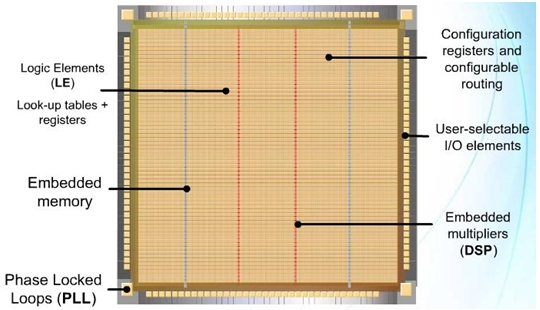
\includegraphics[scale=0.5]{fpga.jpg}
	\end{center}
    %EXEMPLO DE REFERENCIA
	\legend{Fonte: \cite{arquiteturafpga}}
\end{figure}

A arquitetura de um FPGA, a qual pode ser observada na Figura  \ref{fig_arquiteturafpga}, é em sua grande maioria composta por Elementos Lógicos (\textit{LE, Logic Elements}), aparelhados em malhas ao longo de todo o equipamento. Separam-se os elementos lógicos em dois tipos de unidades: \textit{Look-Up Tables (LUT)}, que implementam funções lógicas mais comuns, como \textit{OR e AND}, e registros que podem implementar lógica síncrona, como \textit{flip-flops}. \cite{arquiteturafpga}

  As memórias embutidas (\textit{Embedded Memory - EM}) podem ser dispostas em série ou paralelo visando obter-se memórias mais robustas. Outros recursos são os multiplicadores embutidos, os quais podem ser cascateados de forma a melhorar o processamento digital de sinais (PDS), colaborando na implementação de funções avançadas.\cite{arquiteturafpga}
 
  Os FPGAs também possuem elementos de entrada e saída, identificados na Figura \ref{fig_arquiteturafpga} por \textit{User-selectable I/O Elements}, que podem ser aparelhados e utilizados a medida que o arquiteto necessite. Estes elementos podem ser posicionados e configurados para comunicar o FPGA com outros dispositivos externos presentes no circuito impresso. \cite{arquiteturafpga} \cite{}
  
\begin{figure}[htb]
	\caption{\label{fig_roteamentofpga}Elementos básicos da arquitetura de roteamento de um FPGA}
	\begin{center}
	    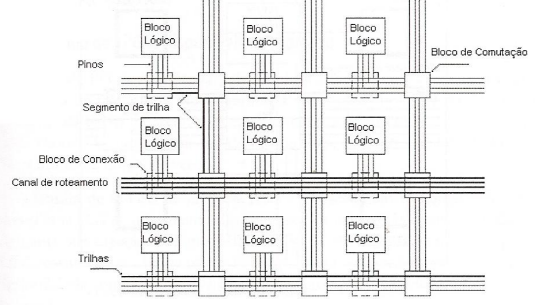
\includegraphics[scale=0.8]{arquiteturaroteamento.PNG}
	\end{center}
    %EXEMPLO DE REFERENCIA
	\legend{Fonte: \cite{logicaprogramavel}}
\end{figure}  
  
  A arquitetura de roteamento de um FPGA, apresentada na Figura \ref{fig_roteamentofpga}, pode ser explicada como a forma organizacional e posicional dos barramentos das chaves de comutação, a qual permite a interconexão entre as células lógicas. \cite{logicaprogramavel}
	
    Segue breve explicação dada em \cite{logicaprogramavel} dos itens dispostos na Figura \ref{fig_roteamentofpga}:
    
\begin{itemize}
\item Pinos: Entrada e Saída de blocos lógicos.
\item Conexão: Ligação elétrica de um par de pinos
\item Rede: Conjunto de pinos que estão conectados.
\item Bloco de Comutação: Utilizado para conectar os segmentos da trilha.
\item Segmentos da Trilha: Segmento não interrompido por chaves programáveis.
\item Canal de Roteamento: Grupo de 2 ou mais 3 trilhas paralelas.
\item Bloco de Conexão: Permite a conectividade das entradas e saídas de um bloco lógico
com os segmentos de trilhas nos canais.
\end{itemize}

\subsection{Dispositivo alvo}
\begin{figure}[htb]
	\caption{\label{fig_fpgaaltera}Elementos básicos da arquitetura um FPGA Altera}
	\begin{center}
	    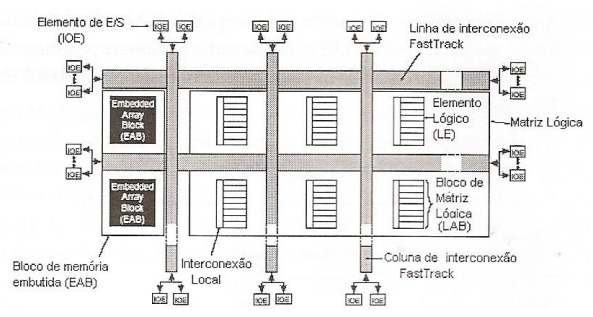
\includegraphics[scale=0.8]{fpgaaltera.PNG}
	\end{center}
    %EXEMPLO DE REFERENCIA
	\legend{Fonte: \cite{logicaprogramavel}}
\end{figure}

A família de FPGAs da Altera Corp. possui como característica uma
hierarquia de três níveis muito similar à encontrada nos \textit{CPLDs}, que são Dispositivos Lógicos Programáveis Complexos, e é baseada em tecnologia SRAM, também possuindo
uma LUT de quatro entradas como seu elemento lógico básico LE.  A arquitetura
interna básica da família Altera, conforme a Figura \ref{fig_fpgaaltera}, contém três tipos de células lógica: Elemento lógico(LE), bloco de matriz lógica (LAB) e bloco de memória embutido (EAB). \cite{logicaprogramavel}

\begin{figure}[H]
	\caption{\label{fig_cyclone4}Elementos físicos da FPGA Cyclone IV}
	\begin{center}
	    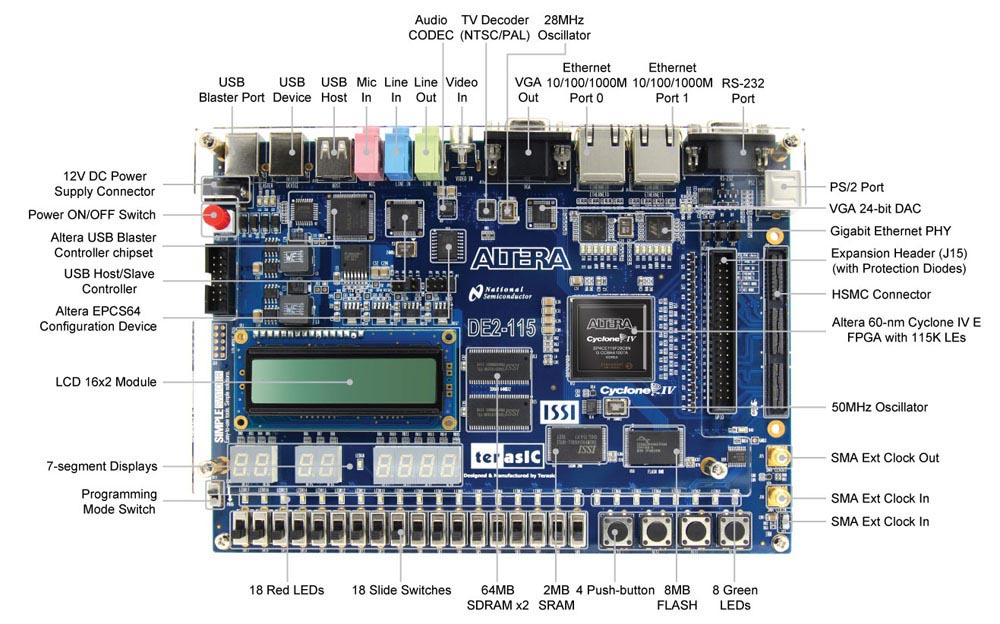
\includegraphics[scale=0.35]{Cyclone4.jpeg}
	\end{center}
    %EXEMPLO DE REFERENCIA
	\legend{Fonte: http://blog.terasic.com/}
\end{figure}

O FPGA Cyclone IV EP4CE30, apresentado na Figura \ref{fig_cyclone4}, possui 28.848 LEs,
memoria dedicada de 594 Kbits, 4 PLLs e 532 pinos de E/S.
Os elementos lógicos presentes na Cyclone IV são divididos em dois modos de operação:
O modo normal é aplicável para aplicações lógicas gerais e funções combinacionais. Nesse modo, 4 entradas de dados proveniente do LAB local interconnect são inseridas em um LUT de 4 entradas. 
O modo aritimetico é ideal para implementação de somadores, contadores, simuladores e comparadores. Um elemento lógico no modo aritimético implementa um somador completo de 2 bits e um \textit{carry chain} básico. \cite{cyclone4altera}



\section{Processo de Síntese}
\subsection{Síntese lógica}
\begin{figure}[htb]
	\caption{\label{fig_sintese}Representação de uma síntese de um circuito}
	\begin{center}
	    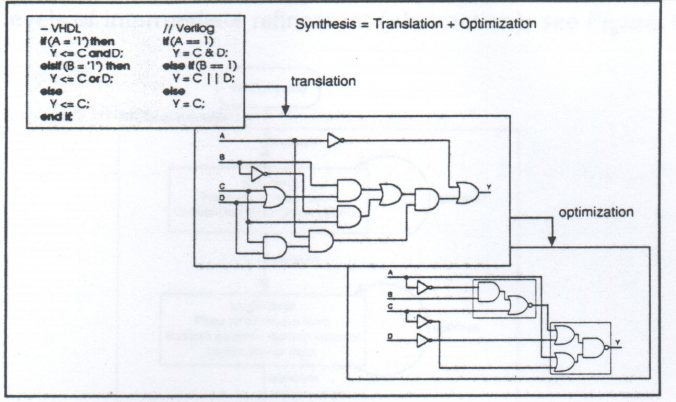
\includegraphics[scale=0.5]{sintese.PNG}
	\end{center}
    %EXEMPLO DE REFERENCIA
	\legend{Fonte: \cite{sintesertl}}
\end{figure}

A Figura \ref{fig_sintese} ilustra uma síntese lógica, a qual é um processo efetuado por ferramentas de síntese, como por exemplo o Quartus, pelo qual o comportamento de uma forma abstrata de circuito, geralmente encontrada em RTL, \textit{register transfer level}, e escrita em linguagens de descrição de hardware, como verilog e vhdl, é gerada uma \textit{netlist}, que é lista de componentes e suas interligações. Tem como objetivo maximizar a performance do circuito, reduzir custos energéticos como também minimizar a área ocupada.

Esse processo, também chamado de fluxo de sintese é dado através de algumas etapas, essas descritas por \cite{sintesertl}:

\begin{itemize}
\item Preparação da descrição do circuito (HDL/VHDL)
\item [Síntese] Tradução para componentes sintéticos (\textit{DesignWare}) e para tecnologia genérica (\textit{GTECH}).
\item Otimização e mapeamento para biblioteca-alvo
\item Síntese de infra-estrutura de teste (\textit{scan})
\item Re-síntese após síntese física
\end{itemize}

\subsection{Síntese Física}

O processo de síntese física de um circuito é a capacidade de se criar um circuito físico a partir de um código RTL. Através desse processo é possível se verificar valores importantes para um circuito, como valores reais de tempo, que podem ser atrelados ao caminho crítico do sistema, que significa o processo mais longo e atrasado que um circuito possui, o qual determina o valor do pulso de relógio no sistema. \cite{sintesefisicahamid}
\begin{figure}[htb]
	\caption{\label{fig_sintesefisica}Representação de uma síntese fisica de um circuito}
	\begin{center}
	    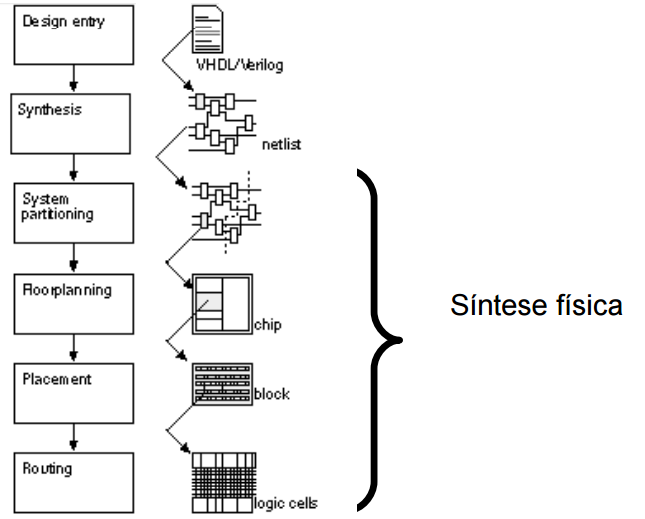
\includegraphics[scale=0.7]{fluxosfisica.png}
	\end{center}
    %EXEMPLO DE REFERENCIA
	\legend{Fonte: \cite{sintesefisica}}
\end{figure}

Assim como a síntese lógica, também é dado através de algumas etapas ilustradas na Figura \ref{fig_sintesefisica}:

\begin{itemize}
\item Partição do sistema
\item \textit{Floorplanning} - Preparação de ambiente
\item \textit{Placement} - Formação de blocos
\item \textit{Routing} - Interligações dos blocos, montando células lógicas
\end{itemize}

% ----------------------------------------------------------
% Metodologia
% ----------------------------------------------------------
\chapter{Descrição do desenvolvimento}
\section{Levantamento de requisitos}

A partir da análise do problema apresentado, percebeu-se a indispensabilidade da aplicação do conceito de paralelismo no processador a ser desenvolvido em virtude da requisição de que 5 instruções fossem executadas simultaneamente a cada ciclo de clock, tirando o máximo proveito dos recursos de hardware. Assim, após uma busca por conceitos acerca da construção de processadores MIPS com paralelismo a nível de instrução, fora reconhecida a inevitabilidade de implementação dos registradores interestágios, responsáveis por todo o processo de funcionamento do pipeline junto a unidade de control do processador.  

Levantou-se também a necessidade de desenvolver estruturas responsáveis para tratar conflitos que seriam provenientes das novas estruturas implementadas responsáveis por dar funcionalidade ao pipeline, seriam estas as unidades de controle de conflito \textit{hazard unit} e \textit{forwarding unit}.

Por conta do tamanho de 8 bits de palavra na memória no padrão MIPS, o qual é seguido pelo processador aqui explanado, e das palavras trabalhadas fora da memória serem de 32 \textit{bits}, avaliou-se a viabilidade da multiplicação do \textit{clock} do processador por 4 no bloco da memória para assim ser possível efetuar as ações de modo sincrono ao sistema.

\section{Principais blocos do \textit{datapath}}
\subsection{Unidade de controle}
\begin{figure}[htb]
	\caption{\label{fig_blococontrol}Bloco da unidade de controle do circuito}
	\begin{center}
	    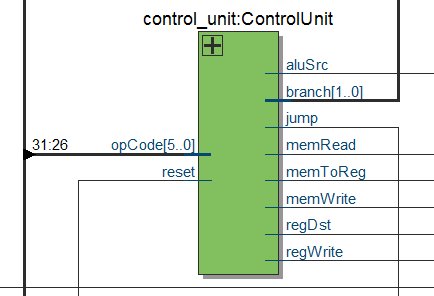
\includegraphics[scale=0.6]{controlunit.PNG}
	\end{center}
    %EXEMPLO DE REFERENCIA
	\legend{Fonte: Proprio autor}
\end{figure}

\begin{table}[htb]
	\caption{\label{tab_tabelacontrol}Sinais da unidade de controle}
	\begin{center}
	    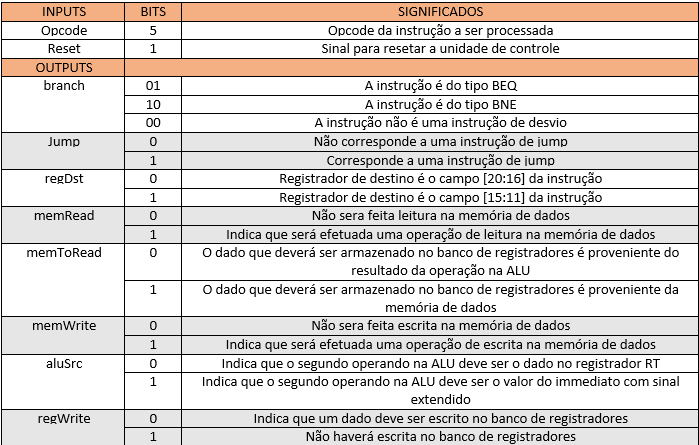
\includegraphics[scale=0.8]{tabela.PNG}
	\end{center}
    %EXEMPLO DE REFERENCIA
	\legend{Fonte: Próprio autor}
\end{table}

A unidade de controle, a qual é apresentada na Figura \ref{fig_blococontrol}, presente no circuito é responsável por controlar as operações do processador. Ela coordena como os estágios de \textit{Pipeline}, a memória de dados, a unidade lógica aritmetica e outras unidades irão corresponder mediante as instruções de um programa. A Tabela \ref{tab_tabelacontrol} apresenta os sinais de controle existentes na unidade de controle essenciais para o funcionamento do sistema.

\subsection{Unidades controladoras de conflitos}
\subsubsection{\textit{Hazard Detection Unit}}


Esta unidade é responsável pela detecção de conflitos estruturais, conflitos de dados e conflitos de controle. No projeto desenvolvido, a memória possui dois canais de leitura, logo o Hazard não tem a necessidade de analizar conflitos estruturais.

	Esta estrutura é responsável por gerar os stalls(bolhas) quando uma instrução buscada tem dependência de uma instrução anterior a ela e esta instrução é uma instrução Load, no caso, é necessário uma bolha pois não seria possível antecipar o dado para a instrução visto que o dado ainda não teria sido carregado da memória.
    
    Quanto ao conflito de controle, essa estrutura verifica se um desvio devido ao branch foi tomado, e ativa os sinais responsáveis por limpar a instrução já buscada(considerando que o desvio não seria tomado) e recarregar a nova instrução no endereço de desvio.
    
    A Figura \ref{fig_blocohazard} representa o bloco \textit{Hazard unit}.

\begin{figure}[H]
	\caption{\label{fig_blocohazard}Bloco de controle de \textit{hazard} no circuito}
	\begin{center}
	    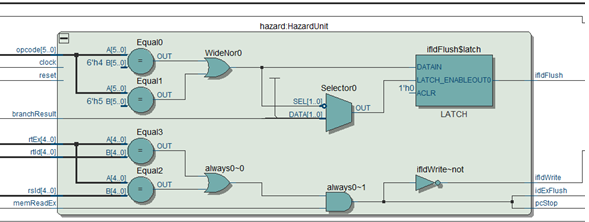
\includegraphics[scale=0.7]{hazardunit.png}
	\end{center}
    %EXEMPLO DE REFERENCIA
	\legend{Fonte: Próprio autor}
\end{figure}

Segue um Pseudo-Código do funcionamento da \textit{Hazard Unit}:

SE: (VaiLerMemoria e ((rsId == rtEx) || (rtId == rtEx)))
  
  ENTÃO:
    
    1. Não atualiza PC
   
   2. Flush em Registradores interestagios IDEX
    
    2. Desabilita escrita em Redistradores interestagios IFID

//Stall em instruções de desvios

SE: (Instrução = BEQ ou Instrução = BNE) E Desvio foi tomado
  
  ENTÃO:
    
    1. Flush em Registradores interestagios IFID
    
    2. Desabilita escrita em registradores IFID

\subsubsection{\textit{Forwarding Unit}}
\begin{figure}[H]
	\caption{\label{fig_blocoforwarding}Bloco da \textit{Forwarding unit} no circuito}
	\begin{center}
	    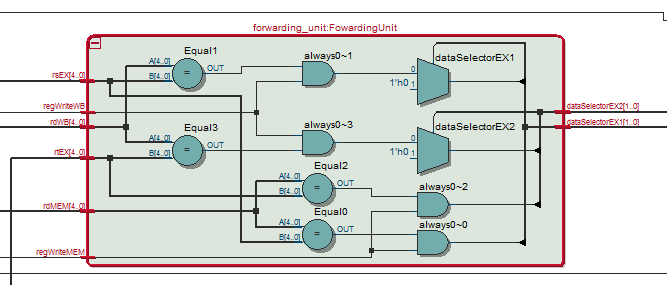
\includegraphics[scale=0.7]{forwardingunit.PNG}
	\end{center}
    %EXEMPLO DE REFERENCIA
	\legend{Fonte: Próprio autor}
\end{figure}

A unidade de adiantamento, cujo bloco é apresentado na Figura \ref{fig_blocoforwarding}, seleciona os \textit{inputs} corretos da ULA do estágio EX e verifica se existe ou não um conflito. Não havendo, os operandos da unidade lógica aritmética virá do banco de registradores, no entanto, caso exista um conflito, os dados destinados à ULA serão provenientes do registrador interestágio EX/MEM ou MEM/WB. Esse controle é dado a partir de seletores nomeados dataSelectorEX1 e dataSelectorEX2, ambos com 2 bits.


Segue um Pseudo-Código da \textit{Forwarding Unit} para ilustrar melhor seu funcionamento:

//Antecipação de dados para RS

SE: EstagioMemVaiSalvarEmBancoDeRegistradores E rsEX == rdMEM
  
  ENTÃO:
    
    1. Antecipar Dado RS do estagio MEM para estagio EX

SE NÃO, CASO:  EstagioWBVaiSalvarEmBancoDeRegistradores E rsEX == rdWB
  
  ENTÃO
   
   1. Antecipar Dado RS do estagio WB para estagio EX

SE NÃO:
   
   1. Não Antecipar dados

//Antecipação de dados para RT
  
  VIDE RS

\subsection{Memória}

O Quartus possui a funcionalidade de identificar um template padrão de memória de modo que a memória descrita em verilog seja assimilada pela placa e, ao invés de sintetizar utilizando suas LEs internas, ele redireciona para a interna da placa.

A estrutura interna da memória segue os requisitos do projeto e, portanto a arquitetura do MIPS, onde cada linha da memória possui 1 byte e o seu endereçamento é a partir de uma palara de 2 bytes.

Uma vez que a memória era compartilhada, a memória possui dois barramentos de entrada e dois barramentos de saída, ambos de 32 para evitar conflito de dados entre os estágios de Instruction Fetch e Memory. A figura~\ref{fig_blocomemoria} exibe o bloco de memória sintetizado pelo quartus, com as suas respectivas entradas e saídas.

\begin{figure}[H]
	\caption{\label{fig_blocomemoria}Bloco de memória no circuito}
	\begin{center}
	    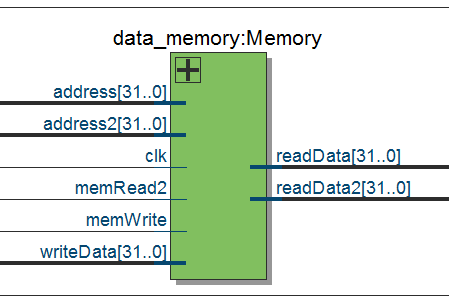
\includegraphics[scale=0.8]{memoria.PNG}
	\end{center}
    %EXEMPLO DE REFERENCIA
	\legend{Fonte: Próprio autor}
\end{figure}

Uma vez que a memória e o processador tem tamanhos de palara diferentes (a memória trabalha com palavras de 1 byte e o processador com palavras de 4 byts), houve a necessidade de se criar uma estrutura anexa a estrutura de memória de maneira que os dados oriundos do processador pudessem ser armazenados na memória sem erros.

Para realizar esta função foi criado um acumulador, com o clock 10 vezes mais rápido do que o clock do sistema (o aumento do clock acontece para que os dados já estejam prontos quando o clock do sistema pulsar). Seu objetivo era capturar as palavras de 4 bytes que chegavam para ser gravadas na memória, dividi-las em 4 partes e gravar cada parte em uma linha da memória, já para a saída o acumulador capturava 4 linhas consecutivas e formava a palavra de 4 bytes necessárias para a leitura da cpu. A Figura ~\ref{fig_statemachinememory} exibe o diagrama de estados da máquina responsável por acumular os dados.

\begin{figure}[H]
	\caption{\label{fig_statemachinememory}Ilustração da máquina de estados da memória}
	\begin{center}
	    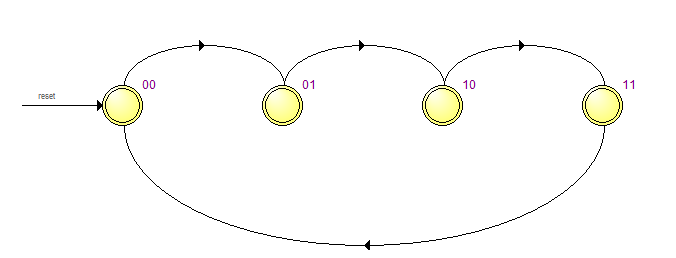
\includegraphics[scale=0.7]{statemachinememory.PNG}
	\end{center}
    %EXEMPLO DE REFERENCIA
	\legend{Fonte: Próprio autor}
\end{figure}

% ----------------------------------------------------------
% Resultados e discussões
% ----------------------------------------------------------
\chapter{Resultados e Discussões}
%Arquivo de test bnench possui dois módulos principais o da memória e o da CPU estes arquivos são interligados e vai verificar os resultados através do arquivo de testes que é passado como parâmetro, o arquivo (passado como parâmetro) vai mostar em cada ciclo de clock quais os estado e  quais os dados que estão em cada um desses estágios sendo possível verificar os erros que estão tendo como erros de imediato, de registrador de unidade de controle e etc.%

\subsection{Testes}
\subsubsection{Visão geral}
Com o objetivo de detectar possíveis erros de desenvolvimento das unidades do processador, foram desenvolvidos alguns testes que executavam as funcionalidades destas unidades de maneira individual, ou seja, não automatizadas. As unidades que tiveram testes foram a unidade de controle, o pc e seu respectivo somador, a unidade de lógica aritmética e a cpu em si. Este processo foi essencial para descobrir eventuais erros de lógica e de construção da descrição do circuito.

Pra construir os testes, foram utilizados como base os algoritmos desenvolvidos na etapa anterior do projeto, os seus binários foram gerados pelo montador e inseridos na memória do dispositivo através do comando $readmemb$, para cada ciclo de clock o teste era capaz de exibir todos os dados que estavam em cada pipeline tornando possível a depuração da unidade de controle, unidade de conflitos, unidade de adiantamento, registradores inter-estágios, extensor de sinal e da memória.

\subsubsection{Teste da Unidade de controle}

\begin{figure}[htb]
	\caption{\label{fig_testCpuControl}Teste da unidade de controle no ModelSim}
	\begin{center}
	    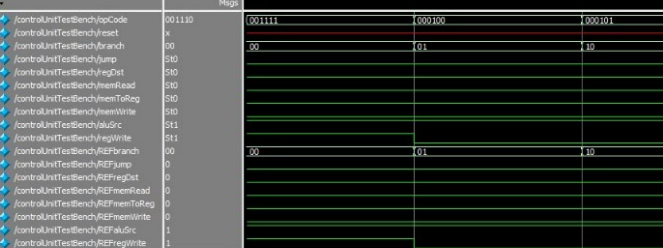
\includegraphics[scale=0.8]{testCpuControl.PNG}
	\end{center}
    %EXEMPLO DE REFERENCIA
	\legend{Fonte: Próprio autor}
\end{figure}

\begin{figure}[htb]
	\caption{\label{fig_testCpuControl2}Teste da unidade de controle no ModelSim - 1}
	\begin{center}
	    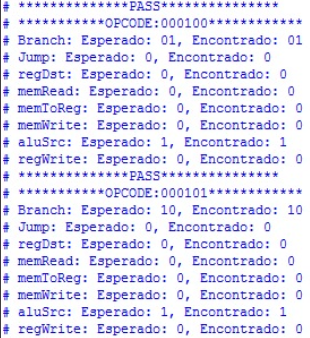
\includegraphics[scale=0.8]{cpucontroltest3.PNG}
	\end{center}
    %EXEMPLO DE REFERENCIA
	\legend{Fonte: Próprio autor}
\end{figure}

O teste da unidade de controle do processador, apresentado nas Figuras  \ref{fig_testCpuControl} e \ref{fig_testCpuControl2}, buscou verificar se os sinais gerados pela unidade através da decodificação do opcode da instrução estavam corretos. Foram feitas entre todos os opcodes possíveis e verificando se a saida do modulo correspondia aos sinais esperados (definidos no teste). Foram encontrados alguns problemas na geração de sinais para instruções de jump, em virtude disso, o teste possibilitou a detecção e correção desse erro, a qual foi executada e a unidade foi aprovada mediante as avaliações.


\subsubsection{Teste da Unidade de controle de PC}

\begin{figure}[H]
	\caption{\label{fig_testPcControl1}Teste da unidade de controle de PC - Testbench}
	\begin{center}
	    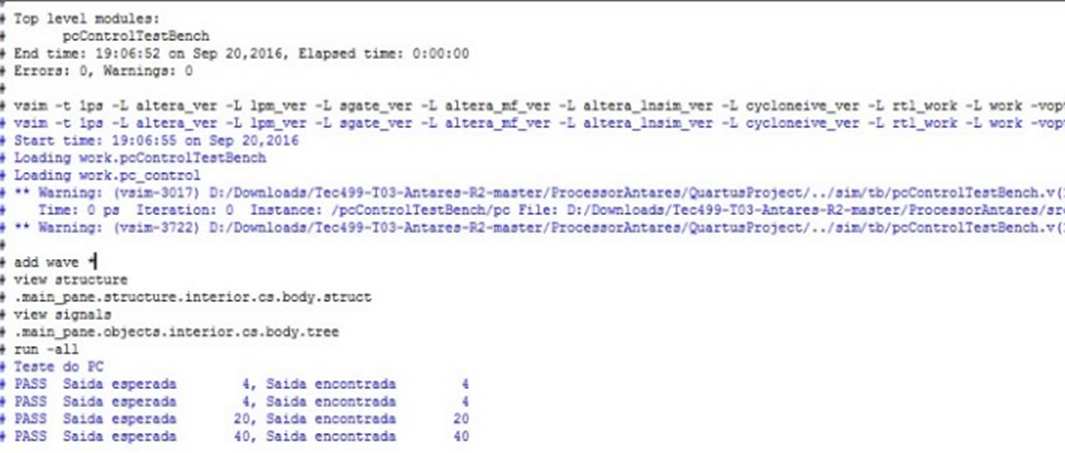
\includegraphics[scale=0.5]{pcControlTestbench.png}
	\end{center}
    %EXEMPLO DE REFERENCIA
	\legend{Fonte: Próprio autor}
\end{figure}


\begin{figure}[H]
	\caption{\label{fig_testPcControl2}Teste da unidade de controle de PC - Modelsim}
	\begin{center}
	    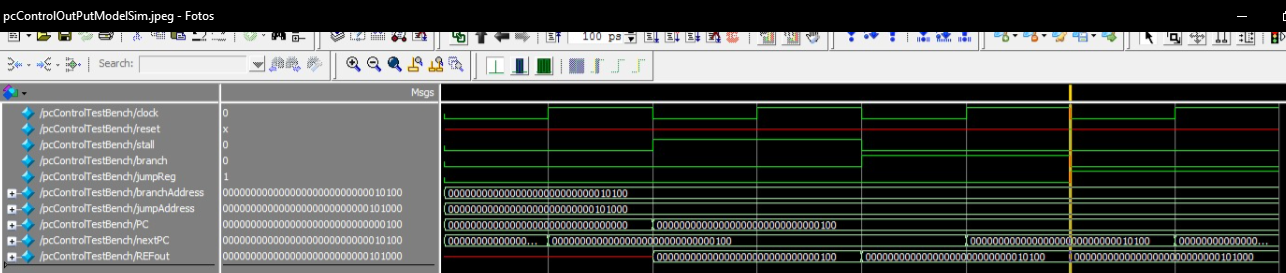
\includegraphics[scale=0.5]{pcControlOutPutModelsim.PNG}
	\end{center}
    %EXEMPLO DE REFERENCIA
	\legend{Fonte: Próprio autor}
\end{figure}

O teste da unidade de controle de PC, podendo ser visualizado através das Figuras \ref{fig_testPcControl1} e \ref{fig_testPcControl2} buscou verificar se os sinais que manipulam o estado do PC, entre eles, sinais de Jump, Branch e Stall, satisfaziam o resultado esperado, que é conferir se o valor do PC após o ciclo era o especificado pelo endereço de branch, endereço de jump, pc anterior +4 ou o mesmo valor. O teste foi feito variando os sinais de controle de entrada e emitindo um pulso de clock.        
        O teste comprovou a exatidão do circuito controlador do program counter(PC) na qual a cada novo ciclo de clock, o valor de PC era atualizado de acordo com seus sinais de controle, ou se mantia o mesmo dependendo do sinal de \textit{Stall}.
        
\subsubsection{Teste da Unidade Lógica Aritmética}
Os testes da unidade lógica aritmética foram feitos através de vetores de testes, testes que geraram valores aleatórios e testes \textit{HardCodes}, visando validar os valores que a ULA estava disponibilizando após seu processamento. Os resultados foram satisfatórios pois obtiveram 100 por cento de exito, comprovando o bom funcionamento dessa unidade, a qual é de extrema importância para o processador.  

\subsubsection{Teste da CPU}
No teste geral do processador existem 2 modulos principais, um modulo da memoria e outro da cpu. Nesse teste é feito uma interligação entre a memória e o processador e verificará os resultados do arquivo de teste que é passado como parâmetro.
Esse processo mostra em cada ciclo de clock quais são os estados e quais são os dados que estão em cada estágio do pipeline, podendo apresentar possíveis erros que possam acontecer em registradores, na unidade de controle e em unidades em geral, pois trata-se de um teste abrangente em termo de quantidade de módulos testados.

\subsection{Síntese lógica do projeto}
Através da síntese lógica do Quartus, foi possível determinar os recursos utilizados pela CPU na FPGA, a descrição do circuito ocupou um total de 482 das 1803 LABs disponíveis (corresponde a 27\%), 6079 das 28848 LEs disponíveis (correspondente a 21\%) destas 4748 geraram circuitos combinacionais sem registradores, 456 foram utilizadas apenas como registradores e 875 como circuitos combinacionais com registradores. Dentre as LEs utilizadas 3322 eram de 4 entradas, 1963 de 3 entradas e 338 com duas ou menos entradas, 4302 dos LEs estavam operando no modo normal e 1321 no modo aritmético


%total de labs é 482 de 1803 = 27%  ; total de les 6079 de 28848 = 21% -> combinacionais sem registradores = 4748 -> apenas registradores 456 -> combinacionais com registrador -> 875 ; LEs com 4 entradas 3322, com 3 entradas 1963, com menos de duas entradas 338 ; dos les 4302 em normal mode e 1321 aritméticos %
% ----------------------------------------------------------
% Conclusão
% ----------------------------------------------------------
\chapter{Conclusão}
O produto resultante de todo o trabalho foi um processador com paralelismo a nível de instrução atrelado a uma memória compartilhada de 64KB. A efetividade do produto não se dá em 100 por cento devido falhas em casos de execução em algumas instruções, tais como instruções de branch que podem ser executadas incorretamente caso a instrução logo anterior use um dos seus registradores de leitura como registrador de destino.

O problema pode ser resolvido inserindo \textit{forwarding} no estagio \textit{Instruction Decode} ou usando o circuito de antecipação de \textit{branch} apenas como um preditor e fazer a operação efetiva do \textit{branch} no estagio EX, onde será possível fazer \textit{forwarding} de acordo com o projeto já implementado.

Vale salientar que através dos testes desenvolvidos, principalmente o teste geral da cpu, é possível detectar tais erros juntos a outros futuros, o que torna totalmente viável a correção e o aprimoramento do produto a curto prazo.

Como requerido no texto prévio de requisição do processador parcial, a cpu desenvolvida só deveria ser capaz de efetuar operações encontradas em testes específicos previamente elaborados pela mesma equipe desenvolvedora do processador, sendo assim, o projeto pode ser bem mais aperfeiçoado através da inserção de novas instruções. Também pode ser considerado um possível trabalho futuro o acréscimo de uma tabela de predição de branch, a qual melhoraria a performance da cpu.
\endgroup

% ----------------------------------------------------------
% Referências bibliográficas
% ----------------------------------------------------------
\bibliography{abntex2-modelo-references}
%---------------------------------------------------------------------
% INDICE REMISSIVO
%---------------------------------------------------------------------
% \phantompart
% \printindex
%---------------------------------------------------------------------

\end{document}
